%%%% utfprpgtex-slides.tex, 2019/02/21
%%%% Copyright (C) 2015-2019 Luiz E. M. Lima (luizeduardomlima@gmail.com)
%%
%% Este arquivo pode ser distribuído e/ou modificado sob as condições da
%% Licença Pública do Projeto LaTeX, tanto a versão 1.3 desta licença ou (à sua
%% opção) qualquer versão posterior.
%% A versão mais recente desta licença está disponível em
%%   http://www.latex-project.org/lppl.txt
%% e a versão 1.3 ou posterior faz parte de todas as distribuições de LaTeX
%% versão 2005/12/01 ou posterior.
%%
%% Este arquivo tem o estado de manutenção da LPPL `mantida'.
%%
%% O mantenedor atual deste arquivo é Luiz E. M. Lima.
%%
%% Este projeto consiste dos arquivos utfprpgtex-slides.sty e
%% utfprpgtex-slides.tex.
%%
%% utfprpgtex-slides.tex é o arquivo principal do modelo LaTeX (não oficial)
%% para produção de apresentação de slides da Universidade Tecnológica Federal
%% do Paraná (UTFPR). Foi desenvolvido baseado no modelo de apresentação de
%% slides do abnTeX2, disponível em <http://www.abntex.net.br/>, criado por
%% Fábio Rodrigues Silva usando a classe beamer, disponível em
%% <http://ctan.org/pkg/beamer/>.

%% Classe e opções de documento
%%%% Modo apresentação --- Descomente o comando \documentclass[]{beamer}
\documentclass[%% Opções
  10pt,%% Tamanho de fonte: 10pt, 11pt, 12pt, etc.
  aspectratio = 169,%% Razão de aspecto: 1610 (16:10), 169 (16:9), 149 (14:9), 54 (5:4), 43 (4:3 - padrão) e 32 (3:2)
  compress,%% Tenta reduzir o tamanho das barras de navegação (comente para desabilitar)
  t,%% Alinhamento vertical dos quadros: b (fundo), c (centro) e t (topo)
  % handout,%% Cria uma versão que usa as especificações de sobreposição do folheto (comente para desabilitar)
]{beamer}%% Classe beamer
%%%% Modo artigo --- Descomente os comandos \documentclass[]{article} e \usepackage{beamerarticle}
% \documentclass[a4paper, twocolumn]{article}%% Classe artigo
% \usepackage{beamerarticle}%% Utiliza o modo artigo da classe beamer

%% Passagem de opções para pacotes
\PassOptionsToPackage{english, main = brazilian}{babel}%% Suporte multilíngue

%% Pacotes utilizados
\usepackage[UseMECLogo]{utfprpgtex-slides}%% Estilos do modelo

%% Arquivo de referências
\addbibresource{utfprpgtex-slides.bib}

%% Arquivos de logomarcas (presentes no diretório ``Logos'') --- Deixe o campo {} vazio ou comente para remover
\logoevent{logo-evento}%% Logomarca do evento
\logoorg{logo-org}%% Logomarca da organização promotora
\logoextinst{logo-inst-ext}%% Logomarca da instituição do autor externo
\logoprog{logo-ppg}%% Logomarca do programa ou do curso
\logodept{logo-da}%% Logomarca do departamento ou da coordenação
\logocampus{logo-utfpr-pg}%% Logomarca do câmpus

%% Informações do documento
\title[Título da Apresentação]{%% Título da apresentação: [curto] e {longo}
  \texorpdfstring{\mode<article>{\bfseries}}{}%% Modo artigo --- Negrito
  Título da Apresentação em Congresso, Seminário ou Evento\\%
  Técnico/Científico ou para Defesa de Trabalho Acadêmico%
}
\subtitle{%% Subtítulo da apresentação
  Subtítulo da Apresentação em Congresso, Seminário ou Evento\\%
  Técnico/Científico ou para Defesa de Trabalho Acadêmico%
}
\subject{Assunto}%% Assunto da apresentação, e.g.: {Nome do Evento}
%%%% Congresso, Seminário ou Evento Técnico/Científico --- Descomente os comandos \author[]{}, institute[]{} e \titlegraphic{}
% \author[P. Autor(a), S. Autor(a), T. Autor(a)]{%% Autor(es): [curto] e {longo}
  % \footnotesize%
  % Primeiro(a) Autor(a)\inst{1}%
  % \And Segundo(a) Autor(a)\inst{2}%
  % \And Terceiro(a) Autor(a)\inst{3}%
% }
% \institute[UTFPR/<INST-EXT>]{%% Instituição(ões): [curto] e {longo}
  % \inst{1,3}\utfprname, Ponta Grossa, Paraná, Brasil%
  % \par\inst{2}<Instituição do(a) Autor(a) Externo(a)>, <Cidade>, <Estado>, <País>%
  % \par e-mail(s): \email[1]{autor1@dominio}%
                  % \sep\email[2]{autor2@dominio}%
                  % \sep\email[3]{autor3@dominio}%
% }
% \titlegraphic{%% Logomarcas do evento
  % \vspace*{-\baselineskip}%
  % \eventlogos%
% }
%%%% Defesa de Trabalho Acadêmico --- Descomente os comandos \author[]{}, institute[]{} e \titlegraphic{}
\author[N. Autor(a)]{%% Autor(a): [curto] e {longo}
  Nome do(a) Autor(a)%
  \authormail{autor@dominio}%
  \advisor{Orientador(a): Prof(a). Dr(a). Nome do(a) Orientador(a)}%
}
\institute[UTFPR-PG/<DEPTO>/<PPG>]{%% Instituição: [curto] e {longo}
  \utfprname, Câmpus Ponta Grossa (UTFPR-PG)%
  \par <Departamento ou Coordenação> (<DEPTO>)%
  \par <Programa ou Curso> (<PPG>)%
}
\titlegraphic{%% Logomarcas da instituição
  \vspace*{-\baselineskip}%
  \institutelogos%
}
\campus{PG}{Câmpus Ponta Grossa}%% Câmpus: {sigla} e {nome} --- Modo artigo
\departamento[logo-da]{<DEPTO>}{%% Depto., Coord., Prog. ou Curso: [logo], {sigla} e {nome} --- Modo artigo
  Departamento Acadêmico de <Nome do Depto.>%
}
\date[\today]{}%% Data: [curto] e {longo}

%% Início do documento
\begin{document}

\mode<presentation>{%% Modo apresentação --- Páginas de título e de sumário
  \frame{\titlepage}%
  \begin{frame}{Sumário}{~}%
  \tableofcontents[pausesections]%
  \end{frame}%
}

\mode<article>{%% Modo artigo --- Página de título
  \maketitle%
  \thispagestyle{firstpagestyle}%
}

\section{Introdução}\label{sec:intro}

\begin{frame}{\sectiontitle{sec:intro}}{Subtítulo da seção ou do slide}
Esta apresentação de slides foi desenvolvida com base na classe \LaTeX/Beamer, disponível em <\url{http://www.ctan.org/pkg/beamer}>.
\begin{block}{Citações e referências}
\begin{itemize}
\item Exemplos de referências podem ser observados nas citações:
\begin{itemize}
\item Implícita: ... \cite{Nriagu1988,Lamport1994,VanEkenstein1997}.
\item Explícita: Segundo \textcite{Wizentier1992,Faina2000},...
\end{itemize}
\item Citações e referências podem ser inseridas neste documento usando os comandos do pacote \LaTeX\ ``biblatex'', disponível em <\url{http://ctan.org/pkg/biblatex/}>.
\item Os dados de cada referência podem ser obtidos de um arquivo ``bibtex'' (*.bib), geralmente na própria página de \textit{download} da referência (artigos, livros, etc.), ou no Google Acadêmico, etc.
\item Para gerar ou editar entradas de arquivos ``bibtex'' (*.bib) pode-se utilizar a ferramenta ``Bibtex Editor'', disponível em <\url{http://truben.no/latex/bibtex/}>, ou ``ZoteroBib'', disponível em <\url{http://zbib.org/}>, dentre outras.
\end{itemize}
\end{block}
\end{frame}

\section{Revisão da Literatura}\label{sec:revlit}

\begin{frame}{\sectiontitle{sec:revlit}}{Subtítulo da seção ou do slide}
\begin{block}<+->{Exemplo de lista de itens}
\begin{itemize}
\item Item a.
\item Item b.
\item Item c.
\end{itemize}
\end{block}
\begin{block}<+->{Exemplo de lista de itens numerada}
\begin{enumerate}[<+-|alert@+>]
\item Item numerado 1.
\item Item numerado 2.
\item Item numerado 3.
\end{enumerate}
\end{block}
\end{frame}

\begin{frame}[fragile = singleslide]{\sectiontitle{sec:revlit}}{Subtítulo da seção ou do slide}
Uma equação como $y = a x^2 + b x + c$ pode ser inserida ao longo do texto de um parágrafo usando o ambiente \LaTeX\ ``math'' (\verb|$...$|). Por outro lado, a seguinte equação é um exemplo de equação não numerada inserida numa linha em separado usando o ambiente \LaTeX\ ``displaymath'' (\verb|\[...\]|).
\begin{block}{}
\[
\frac{\mathrm{d}y}{\mathrm{d}x} = \gamma \ \mathrm{sen} x
\]
\end{block}
A Equação~\eqref{eq:fx} é um exemplo de equação inserida usando o ambiente \LaTeX\ ``equation'' e numerada automaticamente.
\begin{block}{}
\begin{equation}\label{eq:fx}
f(x) = \frac{1}{\alpha} \int^L_0 \left(\frac{x^2}{2} - \frac{x^3}{3}\right) \mathrm{d}x
\end{equation}
\end{block}
Para gerar ou editar equações em \LaTeX\ pode-se utilizar a ferramenta ``Formula Sheet'', disponível em <\url{http://formulasheet.com/}>, dentre outras.
\end{frame}

\section{Material e Métodos}\label{sec:matmet}

\begin{frame}{\sectiontitle{sec:matmet}}{Subtítulo da seção ou do slide}
\begin{columns}[t]
\column{0.475\textwidth}
A Figura~\ref{fig:campuspontagrossa} é um exemplo de figura inserida usando o ambiente \LaTeX\ ``figure'' e numerada automaticamente.
\begin{figure}[!htb]
\centering
\caption{Exemplo de legenda de figura.}
\label{fig:campuspontagrossa}
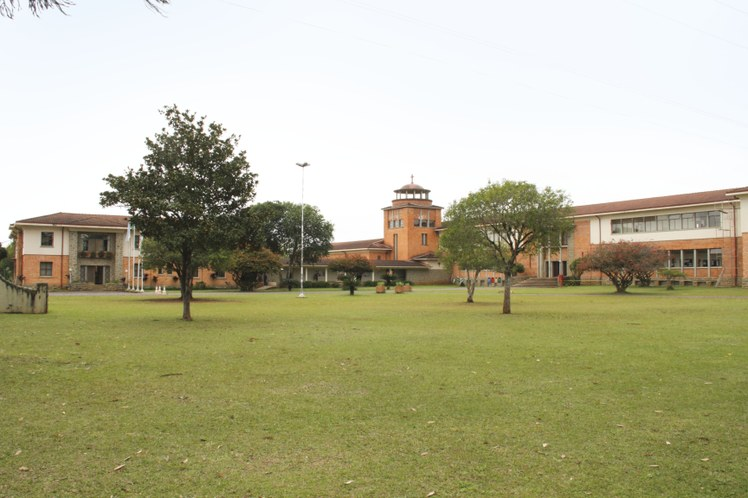
\includegraphics[width = 0.75\columnwidth]{./Figuras/campuspontagrossa}
\source{\textcite{UTFPR2018}.}
\end{figure}
\mode<article>{\\}%% Modo artigo --- Quebra de linha
\column{0.475\textwidth}
Atalhos para execução de arquivos (externos) também podem ser inseridos, conforme exemplo na sequência.
\begin{block}{Exemplo de atalho para vídeo}
\linktofile{./Videos/experimentofluido.flv}{Experimento de mecânica dos fluidos (vídeo).}
\end{block}
\end{columns}
\end{frame}

\begin{frame}{\sectiontitle{sec:matmet}}{Subtítulo da seção ou do slide}
\begin{columns}[t]
\column{0.375\textwidth}
A Tabela~\ref{tab:Ldimensoes} é um exemplo de tabela inserida usando o ambiente \LaTeX\ ``table'' e numerada automaticamente.
\begin{table}[!htb]
\centering
\mode<presentation>{\scriptsize}%% Modo apresentação --- Tamanho de fonte
\mode<article>{\small}%% Modo artigo --- Tamanho de fonte
\caption{Exemplo de legenda de tabela.}
\label{tab:Ldimensoes}
\begin{tabular*}{\columnwidth}{@{\extracolsep{\fill}}llll}
\hline
$L$   & $L^2$     & $L^3$     & $L^4$     \\
{[m]} & {[m$^2$]} & {[m$^3$]} & {[m$^4$]} \\ \hline
1     & 1         & 1         & 1         \\
2     & 4         & 8         & 16        \\
3     & 9         & 27        & 81        \\
4     & 16        & 64        & 256       \\
5     & 25        & 125       & 625       \\ \hline
\end{tabular*}
\source{Autoria própria.}
\end{table}
\mode<article>{\\}%% Modo artigo --- Quebra de linha
\column{0.575\textwidth}
Para gerar ou editar tabelas em \LaTeX\ pode-se utilizar a ferramenta ``Tables Generator'', disponível em <\url{http://www.tablesgenerator.com/}>, dentre outras.
\begin{block}{Informações e dicas sobre \TeX/\LaTeX}
\begin{itemize}
\item \LaTeX\ Project: <\url{http://www.latex-project.org/}>.
\item Comprehensive \TeX\ Archive Network (CTAN): <\url{http://www.ctan.org/}>.
\item \TeX\ Users Group (TUG): <\url{http://www.tug.org/}>.
\item \LaTeX\ - Wikibooks: <\url{http://en.wikibooks.org/wiki/LaTeX/}>.
\item \TeX\ - \LaTeX\ Stack Exchange: <\url{http://tex.stackexchange.com/}>.
\end{itemize}
\end{block}
\end{columns}
\end{frame}

\section{Resultados e Discussão}\label{sec:resdisc}

\begin{frame}{\sectiontitle{sec:resdisc}}{Subtítulo da seção ou do slide}
As Figuras~\ref{fig:graficoxy1} e \ref{fig:graficoxy2} são mais exemplos de figuras inseridas usando o ambiente \LaTeX\ ``figure'' e dispostas em duas colunas.
\begin{columns}[t]
\column{0.475\textwidth}
\begin{figure}[!htb]
\centering
\caption{Exemplo de legenda de figura.}
\label{fig:graficoxy1}
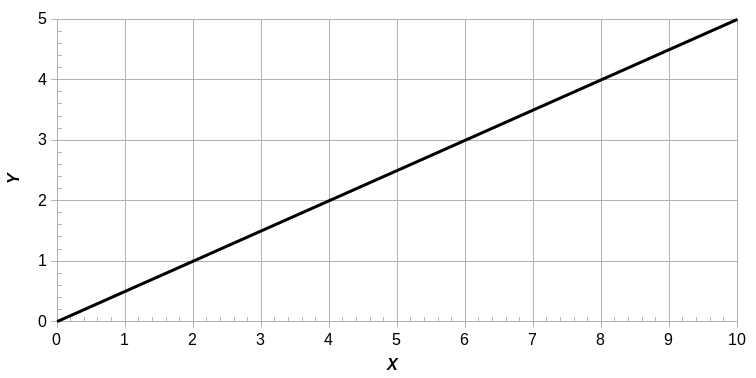
\includegraphics[width = 0.8\columnwidth]{./Figuras/graficoxy}
\source{Autoria própria.}
\end{figure}
\column{0.475\textwidth}
\begin{figure}[!htb]
\centering
\caption{Exemplo de legenda de figura.}
\label{fig:graficoxy2}
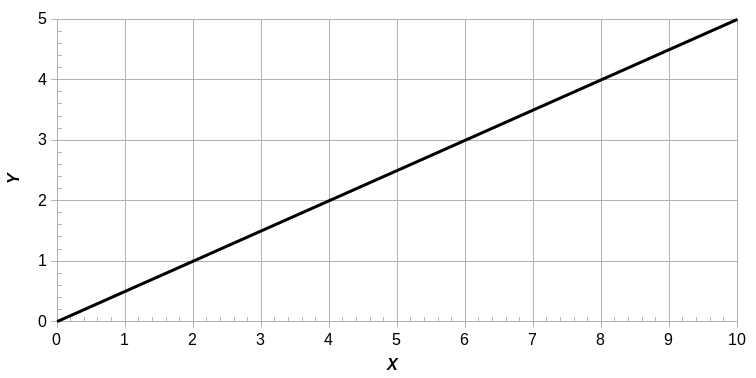
\includegraphics[width = 0.8\columnwidth]{./Figuras/graficoxy}
\source{Autoria própria.}
\end{figure}
\end{columns}
\end{frame}

\section{Conclusões}\label{sec:concl}

\begin{frame}{\sectiontitle{sec:concl}}{Subtítulo da seção ou do slide}
\begin{block}{Lista de conclusões}
\begin{itemize}
\item Conclusão 1.
\item Conclusão 2.
\item Conclusão 3.
\item Conclusão 4.
\item Conclusão 5.
\end{itemize}
\end{block}
\end{frame}

\mode<presentation>{%% Modo apresentação --- Referências
  \section{Referências}\label{sec:ref}%
  \begin{frame}[allowframebreaks]{\sectiontitle{sec:ref}}{~}%
  \printbibliography[heading = none]%
  \end{frame}%
}

\mode<article>{\printbibliography}%% Modo artigo --- Referências

\section*{Agradecimentos}\label{sec:agrad}

\begin{frame}[c]{\sectiontitle{sec:agrad}}{\mode<presentation>{~}}
Pelo apoio recebido para o desenvolvimento deste trabalho e a participação neste evento:
\mode<presentation>{\vfill}%% Modo apresentação --- Espaçamento vertical
\begin{center}

\includegraphics[height = \logoheight]{./Logos/logo-capes}
\hfill

\includegraphics[height = \logoheight]{./Logos/logo-cnpq}
\hfill

\includegraphics[height = \logoheight]{./Logos/logo-fa}
\mode<presentation>{\vfill}%% Modo apresentação --- Espaçamento vertical

\includegraphics[height = \logoheight]{./Logos/logo-utfpr}
\end{center}
\end{frame}

\mode<presentation>{%% Modo apresentação --- Agradecimentos
  \begin{frame}[c]{\sectiontitle{sec:agrad}}{~}%
    \vfill%
    \begin{center}%
      \begin{Huge}%
        Por sua atenção!!!%
      \end{Huge}%
    \end{center}%
    \vfill%
    \begin{block}{Declaração de Responsabilidade}%
      O(s) autor(es) é(são) o(s) único(s) responsável(eis) pelo material impresso contido neste documento.%
    \end{block}%
  \end{frame}%
}

\mode<article>{%% Modo artigo --- Declaração de responsabilidade
  \section*{Declaração de Responsabilidade}%
  O(s) autor(es) é(são) o(s) único(s) responsável(eis) pelo material impresso contido neste documento.%
}

%% Fim do documento
\end{document}
